\documentclass[11pt]{article}

\usepackage[margin=1in]{geometry}
\usepackage[utf8]{inputenc}
\usepackage[T1]{fontenc}
\usepackage{times}
\usepackage{amsmath,amssymb}
\usepackage{graphicx}
\usepackage{booktabs}
\usepackage[round]{natbib}
\usepackage{hyperref}
\usepackage{xcolor}
\usepackage{enumitem}
\usepackage{microtype}
\usepackage{titling}
\usepackage{framed}

\setlength{\droptitle}{-1cm}
\pretitle{\begin{center}\Large\bfseries}
\posttitle{\end{center}\vspace{0.3cm}}

\hypersetup{
  colorlinks=true,
  linkcolor=black,
  citecolor=blue!50!black,
  urlcolor=blue!50!black
}
\setlist{itemsep=2pt,topsep=3pt}

\title{The Compute--Retrieve Axis Separates Prompt Types, Not Processes:\\ Original Results, Confounds, and a Preregistered Causal Test}

\author{
  Sam Ramdan\\
  Independent Researcher\\
  \texttt{sr4729820@gmail.com}\\[4pt]
  {\small Version 2 (Zenodo v4). Version 1: \href{https://doi.org/10.5281/zenodo.19455724}{doi:10.5281/zenodo.19455724} (Zenodo v1--v3)}\\
  {\small Code and data: \url{https://github.com/Somebodyhere101/compute-retrieve}}
}
\date{October 2026}

\begin{document}

\maketitle

\begin{framed}
\noindent\textbf{What changed in version 2.}
Version~1 was the author's first preprint. It was posted on Zenodo as three uploads on 6--7 April 2026, labelled v1--v3; this paper calls them version~1, and this revision is Zenodo v4. It reported that a single direction in transformer hidden states, the compute--retrieve (CR) axis, detects whether a model is computing or retrieving. Its results on prompt types still stand as reported, but two later tests, one of them preregistered, show that its central interpretation does not hold once prompt format is controlled:
\begin{itemize}
  \item Under exact format and length matching, the axis tracks context vocabulary more than retrievability (Section~\ref{sec:matched}; \citealp{ramdan2026fingerprint}).
  \item In a preregistered causal test in four models, the axis does not follow, and pushing along it barely moves, the depth at which an arithmetic answer settles. Where pushing it changes behaviour, it switches the reply between showing working and stating the answer, and a direction built from the same prompts \emph{without} their labels does the same (Section~\ref{sec:causal}).
\end{itemize}
Version~2 keeps every version-1 number (Section~\ref{sec:original}), adds both tests, revises the title, abstract and conclusions, and replaces the version-1 claims about ``reasoning mode'' and ``failure type'' with claims about prompt type and reply format. A full changelog is in Appendix~\ref{app:changelog}.
\end{framed}

\begin{abstract}
A single mean-difference direction in transformer hidden states, the compute--retrieve (CR) axis, separates computation-heavy prompts (GSM8K-style word problems) from retrieval-heavy prompts (MMLU-style questions) at AUC~$\geq$~0.988 in twelve models from five families. Version~1 of this paper interpreted it as a detector of the model's \emph{computational mode}. We test that interpretation directly.
First, under exact format and length matching, the axis reversed in three of five small Qwen3 base models, and 64--87\% of the reversed gap came from context vocabulary \citep{ramdan2026fingerprint}.
Second, in a preregistered causal test in Qwen3-1.7B, Qwen2.5-7B-Instruct, Qwen3-8B and Qwen3-14B, on multiplication problems of identical format and length, an item's position on the axis does not correlate with how deep in the network its answer settles (Spearman $\rho$ between $-0.03$ and $+0.07$). Pushing the hidden state one calibration gap along the axis shifts settling by at most 0.76 of a layer relative to random pushes that change the output distribution as much. It never shifts settling more than a within-class \emph{length} direction built from the same calibration prompts without their labels. In two models the push switches the reply between showing working and stating the answer (answer-first replies $+0.47$ and $+0.20$), but the length direction does the same or more.
Under the preregistered decision rule, the axis does not track the process within format in any of the four models. Exploratory analyses replicate the axis's difficulty gradient on bare arithmetic ($r$~=~0.83--0.89, partial $r$~=~0.65--0.73 controlling for digit count), find that the length direction separates novel from familiar problems better than the axis (AUC $\approx$~0.84 vs.\ $\approx$~0.63 in three of four models), and read the axis through a Jacobian lens as ``calculate'' versus ``answer''. A preregistered follow-up in Qwen3-8B shows that this readable component is causally inert: the format switch runs through the rest of the axis and survives removal of the lens's workspace.
The CR axis is a reliable detector of prompt type and, in some models, a handle on reply format. It is not a detector of the computation a model performs.
\end{abstract}

\section{Introduction}

Answering ``What is the capital of France?'' and answering ``What is 347~+~289?'' plausibly involve different internal processes: one recalls a stored fact, the other computes a new result. Version~1 of this paper \citep{ramdan2026crv1} reported that one linear direction in hidden-state space, the normalised difference between mean activations on computation and retrieval prompts, separates the two prompt types in every model tested. It interpreted that direction as a detector of the model's computational \emph{mode}, and used it to classify wrong answers on MMLU as ``reasoning errors'' or ``retrieval errors''.

Version~1 also stated its main limitation: the axis \emph{correlates} with prompt type, but it was not shown to track or drive the process. Its own discussion named the missing experiment, which was to shift a model along the axis and observe changed outputs. Five intervention attempts had failed. A second limitation was that every control compared prompts that differ in type, so the axis could be tracking how a prompt looks (its length, vocabulary, or the kind of reply it calls for) rather than what the model does with it.

Version~2 runs the missing tests. It defines the process from what the model does, not from the prompt label. The measures are how deep in the network the answer settles (logit lens; \citealp{nostalgebraist2020logitlens}), what kinds of errors it makes \citep{campbell1985mental}, and whether it shows its working. The stimuli are arithmetic problems whose format and length are identical. The interventions are compared against random pushes of the same output size and against a \emph{label-free} nuisance direction built from the axis's own calibration prompts.

\paragraph{Summary of revised claims.}
(1) The original separation results stand as descriptions of prompt types (Section~\ref{sec:original}).
(2) Under matched format the axis follows vocabulary and wrapper more than retrievability (Section~\ref{sec:matched}).
(3) In four models it neither tracks nor drives where an arithmetic answer settles, and its behavioural effect, where there is one, is a reply-format switch shared with a length direction (Section~\ref{sec:causal}).
(4) The difficulty gradient replicates and is not only a digit-count effect, but with format fixed the axis is a weak detector of familiarity (Section~\ref{sec:explore}).
(5) Version~1's failure-classification result should be read as separating wrong answers by the type of question, not by the process that failed.

\section{The Detector}\label{sec:method}

\paragraph{Axis.} For a model with $L$ blocks, $\mathbf{h}_l(p)$ is the output of block $l$ at the last token of prompt $p$. With computation prompts $\mathcal{C}$ and retrieval prompts $\mathcal{R}$, the CR axis is
\begin{equation}
\hat{\mathbf{a}} = \frac{\bar{\mathbf{h}}_{\mathcal{C}} - \bar{\mathbf{h}}_{\mathcal{R}}}{\|\bar{\mathbf{h}}_{\mathcal{C}} - \bar{\mathbf{h}}_{\mathcal{R}}\|},
\qquad \text{proj}(p) = \mathbf{h}_l(p)\cdot\hat{\mathbf{a}},
\label{eq:axis}
\end{equation}
following representation engineering \citep{zou2023representation}. Positive projections are called ``compute'', negative ``retrieve''.

\paragraph{Calibration and layer.} 30 GSM8K questions \citep{cobbe2021gsm8k} and 30 MMLU questions \citep{hendrycks2021mmlu}, wrapped in the model's chat template where it has one. The layer is the one with the highest calibration AUC among four candidates at about 25\%, 50\% and 75\% of depth and $L-2$. On Gemma~4~E2B, 5-fold cross-validation selects the same layer in every fold (test AUC $0.994\pm0.011$). Fifteen prompts per class give a direction within cosine 0.94 of the full-data axis. Calibration takes 1.6\,s for 60 prompts on one GPU; detection is one forward pass and one dot product.

\paragraph{Gap.} Version~2 adds one quantity: the \emph{gap}, the distance between the two calibration classes along the axis, $\bar{\mathbf{h}}_{\mathcal{C}}\cdot\hat{\mathbf{a}} - \bar{\mathbf{h}}_{\mathcal{R}}\cdot\hat{\mathbf{a}}$. A push of one gap moves a hidden state by as much as the difference between a typical computation prompt and a typical retrieval prompt.

\section{Original Results (Version~1), With Caveats}\label{sec:original}

This section reproduces the version-1 results unchanged. Each subsection ends with how version~2 reads it.

\subsection{Twelve models, five families}

\begin{table}[ht]
\caption{Version~1: the CR axis separates its calibration prompts at AUC~$\geq$~0.988 in twelve models. $d$: Cohen's $d$. Grad $r$: difficulty--projection correlation. $^\ddagger$Validated via controls only.}
\label{tab:models}
\vspace{4pt}
\centering
\small
\begin{tabular}{@{}llcccc@{}}
\toprule
Model & Params & Layer & AUC & $d$ & Grad $r$ \\
\midrule
Pythia-70M & 70M & L1 & 0.988 & 3.13 & 0.27 \\
Pythia-160M & 160M & L3 & 1.000 & 2.95 & 0.62 \\
Pythia-410M & 410M & L6 & 1.000 & 2.82 & 0.51 \\
Pythia-1B & 1B & L4 & 1.000 & 2.94 & 0.28 \\
\midrule
Qwen2.5-0.5B & 0.5B & L12 & 1.000 & 3.95 & 0.84 \\
Qwen2.5-1.5B & 1.5B & L21 & 1.000 & 3.52 & 0.77 \\
Qwen2.5-3B & 3B & L9 & 1.000 & 3.07 & 0.74 \\
Qwen2.5-7B & 7B & L21 & 1.000 & 3.18 & 0.77 \\
\midrule
Gemma-4-E2B & 2.3B & L26 & 1.000 & 3.10 & 0.94 \\
Gemma-4-E4B & 8B & L40 & 0.994 & 3.00 & 0.68 \\
\midrule
Qwen3-30B-A3B & 30B & L36 & 0.997 & 3.50 & 0.85 \\
\midrule
LLaMA-3.2-1B & 1.2B & L12 & 1.000 & $^\ddagger$ & $^\ddagger$ \\
\bottomrule
\end{tabular}
\end{table}

Separation reaches AUC~$\geq$~0.988 in every model (Table~\ref{tab:models}, Figure~\ref{fig:multimodel}), including base models. The difficulty gradient (Section~\ref{sec:v1gradient}) is stronger in instruction-tuned models ($r$~=~0.74--0.94) than in base models ($r$~=~0.27--0.62).

\textit{Version-2 reading.} This shows that GSM8K-style and MMLU-style prompts occupy different regions of hidden-state space, which is not in doubt. In Section~\ref{sec:causal}, recalibrating with the published code gives AUC 0.943--1.000 in four further Qwen models. Qwen2.5-7B-Instruct, the checkpoint version~1 used (Figure~\ref{fig:multimodel}), selects layer 14 with AUC 0.990 here, not layer 21 with 1.000 as in Table~\ref{tab:models}. Version~2 runs in bf16 rather than fp16 and with \texttt{transformers} 5.19 rather than 5.5, and the four candidate layers can swap order when their AUCs are this close.

\begin{figure}[t]
\centering
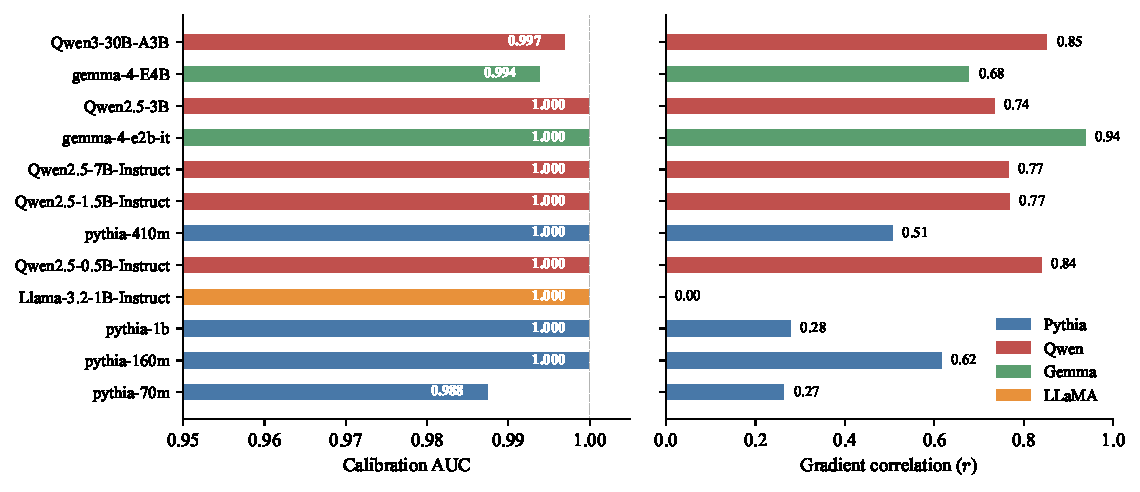
\includegraphics[width=0.85\textwidth]{figures/fig7_multimodel.pdf}
\caption{Version~1. All twelve models separate the calibration prompts at AUC $\geq$ 0.988 (left); gradient correlation is stronger in instruction-tuned models (right).}
\label{fig:multimodel}
\end{figure}

\subsection{Benchmarks and controls}

Calibrated on 30 GSM8K and 30 MMLU questions, the axis separates 100 held-out GSM8K and MMLU questions at AUC~=~1.000 ($d$~=~4.05) and AQUA-RAT from OpenBookQA at AUC~=~1.000 ($d$~=~7.80). Within MMLU, reasoning-heavy subjects project above factual subjects at AUC~=~0.927. Eleven controls (Table~\ref{tab:controls}) addressed prompt format, token count, domain, subject identity and architecture.

\begin{table}[ht]
\caption{Version~1 controls (Gemma~4~E2B unless stated).}
\label{tab:controls}
\vspace{4pt}
\centering
\small
\begin{tabular}{@{}llcl@{}}
\toprule
Control & $N$ & Result & Confound addressed \\
\midrule
Format-matched pairs & 35 & 35/35 separated & Prompt format \\
Within-arithmetic & 30 & AUC = 1.000, $d$ = 4.16 & Domain \\
Within-subject (3 subjects) & 90 & AUC = 0.996--1.000 & Subject identity \\
Reversed length & 30 & 30/30, $d$ = 8.48 & Token count \\
Benchmark length corr. & 100 & $r$ = $-$0.089 & Token count \\
Adversarial prompts & 50 & AUC = 0.998 [0.992, 1.000] & Surface features \\
Cross-arch (Qwen 0.5B) & 40 & 20/20 fmt, 20/20 len & Architecture \\
Cross-arch (LLaMA 1B) & 40 & 20/20 fmt, 20/20 len & Architecture \\
Cross-arch (Pythia 410M) & 40 & 3/20 fmt, 20/20 len & Base model \\
Robustness ($n$=15) & 20 trials & cos = 0.94 & Calibration instability \\
Cross-domain & 4 axes & cos = 0.08--0.70 & Direction universality \\
\bottomrule
\end{tabular}
\end{table}

\textit{Version-2 reading.} Every control compares a prompt that calls for a calculation with a prompt that calls for a recalled fact. The two members of each pair differ in what reply they invite (a worked solution or a short answer), even when their length or surface form is matched. The controls therefore rule out some surface confounds. They do not separate ``the model computes'' from ``the prompt calls for a computational reply''. Version~1 already noted that its adversarial computation prompts were longer and more complex than its retrieval prompts. The cross-domain result (arithmetic and logic axes at cosine 0.08 on Gemma) also showed that the direction depends on the calibration set.

\subsection{Difficulty gradient}\label{sec:v1gradient}

Within bare arithmetic in the format ``What is X op Y?'', the projection rises with an ordinal ``memorisation likelihood'' score assigned to 24 prompts (from $1+1$ at 1 to $2468+1357$ at 10). The correlation is $r$~=~0.951 on Gemma~4~E2B (95\% CI [0.890, 0.966]; 0.711 after partialling out token length) and 0.74--0.84 across Qwen2.5 (Figure~\ref{fig:gradient}). It does not extend to GSM8K word problems.

\textit{Version-2 reading.} The score rises with the number of digits, so the gradient mixes familiarity with length. Section~\ref{sec:explore} replicates it in four models and controls for digit count. The gradient survives, but with format and digit count both fixed the axis separates familiar from novel problems only weakly.

\begin{figure}[t]
\centering
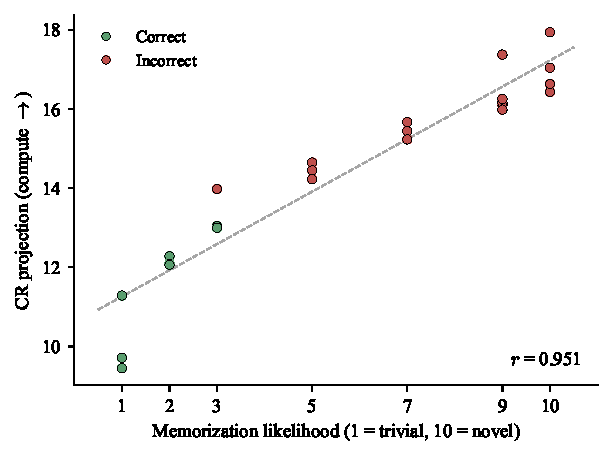
\includegraphics[width=0.6\textwidth]{figures/fig3_gradient.pdf}
\caption{Version~1. CR projection against a memorisation-likelihood score for 24 arithmetic prompts (Gemma~4~E2B, $r$~=~0.951). Green: correct; red: incorrect.}
\label{fig:gradient}
\end{figure}

\subsection{Wrong answers on MMLU}

Among wrong answers to 240 MMLU questions (12 subjects, same multiple-choice format), answers to reasoning-subject questions project above answers to factual-subject questions at AUC~=~0.878 (Gemma-4-E2B, 95\% CI [0.830, 0.917]), 0.885 (Qwen2.5-7B, [0.846, 0.927]) and 0.951 (Qwen3-30B). Version~1 noted that subject is a proxy for failure mode.

\textit{Version-2 reading.} The axis separates these wrong answers by the type of question, as it separates correct ones. Nothing in version~1 or~2 shows that the two groups failed by different processes, so ``failure classification'' should be read as ``question-type classification among errors''.

\subsection{Token dynamics and failed interventions}

During generation, projections on compute tasks stay positive, while on retrieve tasks they start near zero and drift positive ``as the model transitions from stating the answer to explaining it'' (Figure~\ref{fig:trajectories}). Five interventions failed: neuron ablation (output unchanged), self-reflection (sign differs by architecture), output-layer modification (0/11 corrected), gate-pattern transplant (gibberish) and hidden-state injection (no effect). On Qwen~7B, the axis was nearly blind to correctness (AUC~=~0.27), while a truthfulness probe separated the failure groups at AUC~=~0.91, close to the axis's 0.94.

\textit{Version-2 reading.} The drift during explanation is the first sign of what Section~\ref{sec:causal} finds: the axis is sensitive to whether the model is explaining or stating an answer. The injection result is superseded. Added at the detector's layer from the end of the prompt onward, at a size of one calibration gap, the axis does change behaviour in two of four models, but only the reply format.

\begin{figure}[t]
\centering
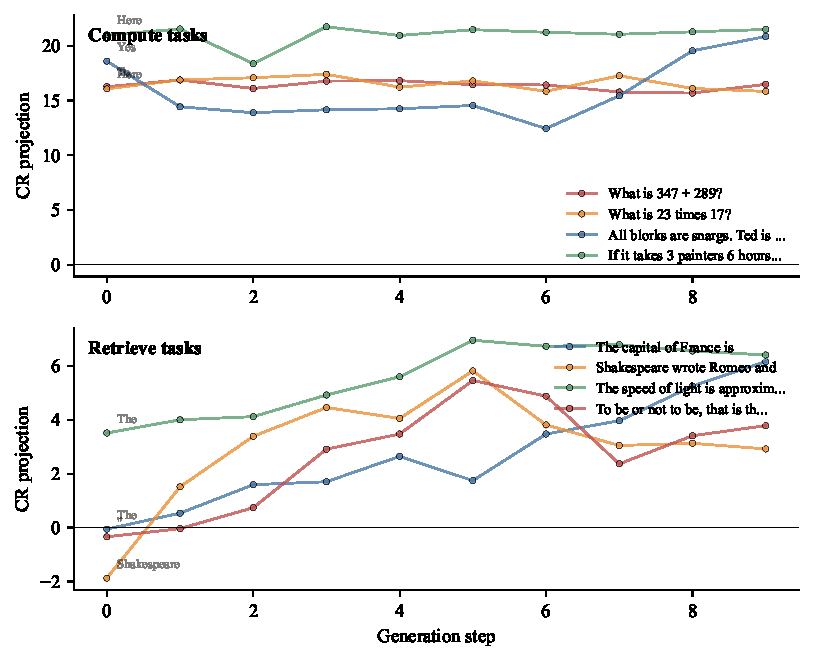
\includegraphics[width=0.8\textwidth]{figures/fig5_trajectories.pdf}
\caption{Version~1. Per-token CR projection during generation. Retrieve tasks drift positive as the model moves from stating an answer to explaining it.}
\label{fig:trajectories}
\end{figure}

\section{What Matched-Format Tests Show}\label{sec:matched}

\citet{ramdan2026fingerprint} (Experiments~5 and~5b) applied the published detector, unchanged, to a contrast that removes length and format differences exactly. In both conditions the model completes a word-labelled Cayley table from the same 281-token context with the same query position.
\begin{itemize}
  \item \textbf{Leak:} the answer is retrievable, because an earlier table in the context is the target's own table.
  \item \textbf{Base:} the answer must be inferred, because the earlier table is a different group's.
\end{itemize}
Behaviour confirms the difference: accuracy is 0.53--0.97 in leak and 0.17--0.22 (chance 0.17) in base. The preregistered prediction was that base projects further toward ``compute'' than leak.
\begin{itemize}
  \item The prediction held in \textbf{0 of 5} small Qwen3 models (0.6B--8B). It was significantly \emph{reversed} in three base models ($d$~=~$-1.34$, $-3.08$, $-0.67$), and null in the post-trained 1.7B ($d$~=~$-0.01$) and in 8B-Base.
  \item The sign depended on the prompt wrapper. Without the chat template, base $>$ leak in three models.
  \item An exploratory vocabulary control showed that context vocabulary reproduces 64--87\% of the reversed gap in the three reversed models. With vocabulary held fixed (shuffled answers with identical words), the predicted direction appeared in the post-trained model ($d_z$~=~$+0.36$; $+0.69$ without the template) and, without the template, in all four models tested ($d_z$~=~$+0.33$ to $+1.67$).
\end{itemize}
So the axis carries a small retrievability signal of the right sign, but under exact format matching it is smaller than, and can be reversed by, the vocabulary and repetition of the context. Its sign in base models depends on the wrapper.

\section{A Preregistered Causal Test}\label{sec:causal}

\subsection{Design}

The test was preregistered in two stages. Stage~1 (hypotheses, measures, decision rule) was frozen on 2026-10-14 at 14:47 (+04:00), before any output. Stage~2 (strength grid, sample sizes) was frozen at 15:18, after two pilots on separate items. The SHA-256 of each file is in Appendix~\ref{app:prereg}.

\paragraph{Models.} Qwen3-1.7B, Qwen2.5-7B-Instruct, Qwen3-8B and Qwen3-14B \citep{qwen3,qwen25}, bf16, chat template, Qwen3 with thinking off. For each, the published detector code (commit \texttt{ce0c61f}) was calibrated on its own 60 prompts.

\paragraph{Items.} All items use the gradient's format, ``What is $a$ * $b$?''.
\begin{itemize}
  \item \textbf{F:} 36 single-digit facts ($2$--$9 \times 2$--$9$).
  \item \textbf{M:} 240 two-digit $\times$ two-digit problems: 60 \emph{familiar} (squares, multiples of 10, or an operand of 11, 25 or 75) and 180 \emph{novel}. Every M prompt has the same format and the same number of tokens.
\end{itemize}

\paragraph{Process measures.} The reply is prefilled with ``$a$ * $b$ = '' and continued greedily.
\begin{itemize}
  \item \textbf{Settling depth $D$.} For each answer digit, the earliest layer from which the logit lens's top token equals the model's output, averaged over the digits and divided by $L$.
  \item \textbf{Error type.} \emph{Recall-type}: the answer to a neighbouring problem, the classic signature of fact retrieval \citep{campbell1985mental}. \emph{Single-digit slip}: one wrong digit, the signature of a procedural error.
  \item \textbf{Shows working $W$.} In free generation (up to 96 tokens), the reply contains a number other than the operands and its final number.
\end{itemize}

\paragraph{Interventions.} A vector is added to the output of the detector's layer at every position from the detector's reading position onward. It is $\pm k$ gaps along the axis, with $k \in \{0.5, 1, 2\}$ and $k=1$ primary.
\begin{itemize}
  \item \textbf{Random controls:} twelve random directions at seven sizes (0.25--4 gaps).
  \item \textbf{Length axis:} the unit average of (long $-$ short) mean differences \emph{within} each calibration class, split at the median token length. It is built from the same 60 prompts without their compute/retrieve labels.
  \item \textbf{Matched-KL comparison:} each push is compared with random pushes that change the output distribution by the same amount (KL summed over the steered continuation), interpolated per item in log KL. An \emph{effect} is the push's change minus that random reference, with a 95\% item-bootstrap interval.
\end{itemize}

\paragraph{Hypotheses (compute = positive).}
\begin{itemize}
  \item \textbf{H1:} within M, projection correlates positively with $D$.
  \item \textbf{H2:} $+1$ gap deepens settling on F.
  \item \textbf{H3:} $-1$ gap makes settling shallower on novel M.
  \item \textbf{H4} (secondary): $-1$ gap raises the share of recall-type errors.
  \item \textbf{H5} (secondary): $+1$ gap raises $W$ on F, and $-1$ gap lowers it on novel M.
  \item \textbf{S:} H2 and H3 exceed the same push along the length axis.
\end{itemize}

\paragraph{Decision rule.} The axis \emph{drives the process} if H2, H3 and S hold in at least two of the three primary models (1.7B, Qwen2.5-7B, 8B); it \emph{tracks but does not drive} if only H1 holds; it \emph{does not track the process within format} if H1 fails.

\paragraph{Deviations.}
\begin{itemize}
  \item \textbf{Size measure.} Stage~1 matched pushes on the KL at the first answer digit. In the pilot that KL was about $10^{-6}$ even when a push changed later digits, so Stage~2 switched to KL over the whole continuation. The Stage-1 version is reported as a sensitivity analysis (Appendix~\ref{app:full}); it changes no conclusion.
  \item \textbf{Prefill.} The prefill ends in a space, because the tokenizer makes the space before a number its own token.
  \item \textbf{Parser fix.} During the runs, Qwen3-8B produced a superscript digit that crashed the answer parser. The parser now counts only ASCII digits, which changes nothing for other answers, and the 8B and 14B runs were resumed.
\end{itemize}
Qwen3-14B was a secondary model in Stage~1 and is reported alongside the primary three.

\begin{table}[ht]
\caption{Calibration of the published detector, and clean accuracy.}
\label{tab:cal}
\vspace{4pt}
\centering
\small
\begin{tabular}{@{}lcccccc@{}}
\toprule
Model & Layer & Cal.\ AUC & Gap & cos(axis, length axis) & F correct & novel M correct \\
\midrule
Qwen3-1.7B & 21 of 28 & 0.993 & 222.8 & 0.64 & 100\% & 89\% \\
Qwen2.5-7B-Instruct & 14 of 28 & 0.990 & 18.7 & 0.67 & 100\% & 93\% \\
Qwen3-8B & 18 of 36 & 1.000 & 39.4 & 0.46 & 100\% & 97\% \\
Qwen3-14B & 10 of 40 & 0.943 & 16.5 & 0.76 & 100\% & 100\% \\
\bottomrule
\end{tabular}
\end{table}

\subsection{The axis does not follow settling depth (H1)}

Across the 240 two-digit problems, the correlation between an item's projection and its settling depth is $\rho$~=~$-0.031$ [$-0.167$, $+0.101$] (1.7B), $+0.035$ [$-0.096$, $+0.156$] (Qwen2.5-7B), $+0.073$ [$-0.044$, $+0.196$] (8B) and $+0.025$ [$-0.106$, $+0.152$] (14B). H1 fails in all four (Figure~\ref{fig:tracking}). The length axis, which carries no class information, correlates better in three models: $+0.30$, $+0.32$ and $+0.13$ ($-0.00$ in 14B; exploratory). Calibration already showed that the two directions share much of their geometry (cosine 0.46--0.76, Table~\ref{tab:cal}).

\begin{figure}[t]
\centering
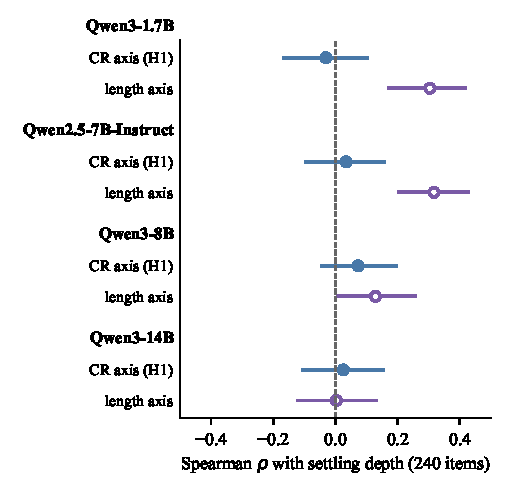
\includegraphics[width=0.48\textwidth]{figures/v2_tracking.pdf}\hfill
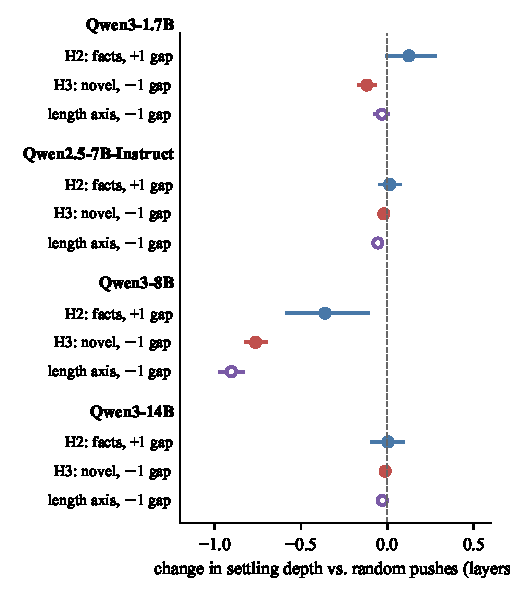
\includegraphics[width=0.48\textwidth]{figures/v2_settling.pdf}
\caption{Left: correlation of axis position (filled) and length-axis position (hollow, exploratory) with settling depth across 240 two-digit problems. Right: change in settling depth, in layers, relative to random pushes of matched KL, for the preregistered pushes (filled) and the same push along the length axis (hollow). Bars: 95\% item-bootstrap intervals.}
\label{fig:tracking}
\label{fig:settling}
\end{figure}

\subsection{Pushing along it barely moves where the answer settles (H2, H3, S)}

\textbf{H2.} A push of one gap toward ``compute'' does not deepen settling on facts more than random pushes of the same KL do: $+0.0045$ [$-0.0000$, $+0.0099$], $+0.0005$ [$-0.0016$, $+0.0027$], $-0.0100$ [$-0.0162$, $-0.0031$] and $+0.0001$ [$-0.0022$, $+0.0022$] of the depth. In Qwen3-8B the effect is reversed.

\textbf{H3.} A push toward ``retrieve'' on novel problems makes settling shallower in two models, 1.7B ($-0.0042$ [$-0.0059$, $-0.0025$]) and 8B ($-0.0212$ [$-0.0228$, $-0.0194$]), and not in Qwen2.5-7B ($-0.0007$) or 14B ($-0.0003$). The largest shift, in 8B, is 0.76 of a layer (Figure~\ref{fig:settling}).

\textbf{S.} Only in 1.7B is the axis's shift larger than the length axis's ($-0.0031$ [$-0.0049$, $-0.0013$]). In Qwen2.5-7B and 8B the length axis moves settling \emph{more} ($+0.0012$ and $+0.0039$, both reversed), and in 14B neither moves it.

\textbf{H4.} Wrong answers are rare after the push (27, 15, 12 and 0 of 180) and none is an answer to a neighbouring problem. The predicted rise in recall-type errors is absent; in 8B the comparison is reversed ($-0.10$ [$-0.13$, $-0.08$]), because random pushes of the same KL cause more errors of every kind.

\textbf{Decision.} H1 fails in all four models. Under the preregistered rule, the axis \emph{does not track the process within format} in Qwen3-1.7B, Qwen2.5-7B-Instruct, Qwen3-8B and Qwen3-14B.

\subsection{Where it changes behaviour, it changes the reply format (H5)}

Unpushed, the models show their working on most novel problems: 100\% (1.7B), 81\% (Qwen2.5-7B), 100\% (8B) and 100\% (14B). Relative to random pushes of the same KL, one gap toward ``retrieve'' changes that share by $-0.004$ [$-0.014$, $+0.002$], $-0.512$ [$-0.544$, $-0.479$], $-0.128$ [$-0.189$, $-0.070$] and $-0.009$ [$-0.024$, $+0.001$]. H5 on novel problems holds in Qwen2.5-7B and 8B. One gap toward ``compute'' raises it in Qwen2.5-7B ($+0.415$ [$+0.392$, $+0.437$]), the only model with room to rise. On single-digit facts, which all models answer directly, a push toward ``compute'' does not make them show working (H5 on facts: not supported in any model; reversed in Qwen2.5-7B, $-0.093$).

The preregistered flag also counts numbers in rambling text after a direct answer. An exploratory measure avoids this: \emph{answers first} means the first number other than the operands is the correct product. One gap toward ``retrieve'' raises it by $+0.467$ [$+0.421$, $+0.511$] in Qwen2.5-7B and $+0.198$ [$+0.142$, $+0.253$] in 8B, and not in 1.7B or 14B (Figure~\ref{fig:format}). For ``What is 72 * 87?'', Qwen2.5-7B-Instruct's unpushed reply begins ``To calculate \(72 \times 87\), you can use the standard multiplication method''. One gap toward ``retrieve'' gives ``The product of 72 and 87 is 6,264.''.

The same push along the length axis does the same thing: $+0.460$ [$+0.417$, $+0.500$] in Qwen2.5-7B and $+0.385$ [$+0.318$, $+0.456$] in 8B. The difference between the axis and the length axis is $+0.007$ [$-0.030$, $+0.043$] and $-0.187$ [$-0.248$, $-0.126$]. One length push gives ``72 multiplied by 87 is 6264.''

\begin{figure}[t]
\centering
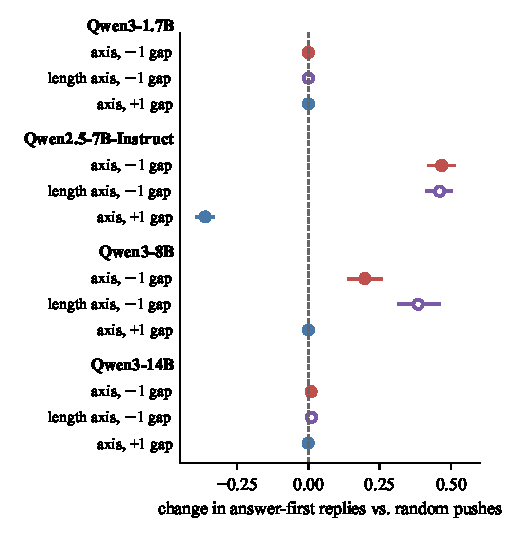
\includegraphics[width=0.48\textwidth]{figures/v2_format.pdf}\hfill
\begin{minipage}[b]{0.48\textwidth}
\caption{Change in answer-first replies on novel two-digit problems relative to random pushes of matched KL (exploratory measure). In Qwen2.5-7B-Instruct and Qwen3-8B, a push toward ``retrieve'' makes the model state the answer instead of working it out. The same push along the label-free length axis (hollow) does as much or more. Bars: 95\% item-bootstrap intervals.}
\label{fig:format}
\vspace{1.2cm}
\end{minipage}
\end{figure}

\begin{figure}[t]
\centering
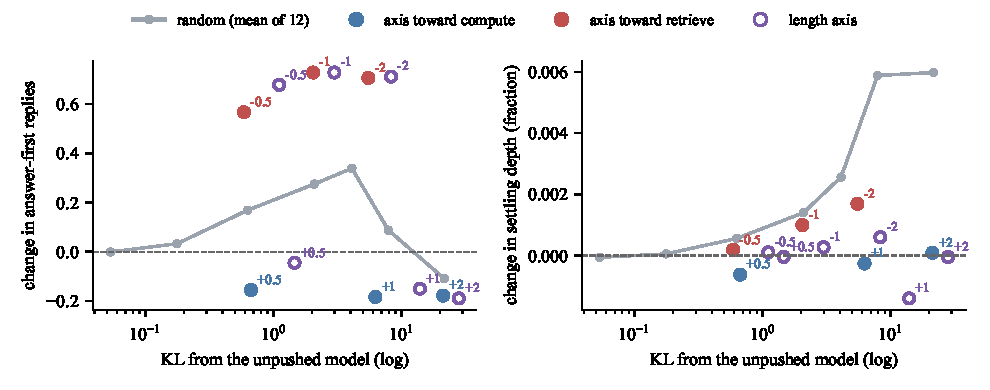
\includegraphics[width=0.95\textwidth]{figures/v2_dose_q25.pdf}
\caption{Qwen2.5-7B-Instruct, novel two-digit problems: change in answer-first replies (left) and settling depth (right) against how much each push changes the output distribution. Random directions (grey) at sizes 0.25--4 gaps; axis and length-axis pushes labelled by size in gaps. The reply format moves far beyond random pushes of the same KL; settling depth does not.}
\label{fig:dose}
\end{figure}

\paragraph{Qwen3-14B.} The detector picks layer 10 of 40 with a weaker calibration (AUC 0.943). Pushes there change the output distribution about as much as in the other models (median KL 0.81 for one gap toward ``retrieve''), but change nothing measured here: settling, accuracy, error type and reply format all stay put.

\section{Exploratory Analyses}\label{sec:explore}

The first three analyses were added after the main results and are exploratory. The last is a separately preregistered follow-up.

\paragraph{The gradient replicates, and is not only digit count.} On version~1's 24 gradient items, the projection correlates with the memorisation score at $r$~=~0.894 (1.7B), 0.853 (Qwen2.5-7B), 0.834 (8B) and 0.870 (14B). With digit count partialled out of both, $r$~=~0.731, 0.705, 0.646 and 0.719 (24 items).

\paragraph{But with format fixed, it is a weak familiarity detector.} Among the 240 two-digit problems, which share format and length, the axis separates novel from familiar problems at AUC 0.61 [0.51, 0.70], 0.62 [0.54, 0.71], 0.65 [0.56, 0.73] and 0.80 [0.72, 0.87]. The length axis does it at 0.85 [0.78, 0.91], 0.83 [0.76, 0.89], 0.85 [0.78, 0.92] and 0.77 [0.70, 0.85]. It is clearly better in the three smaller models, and about as good in 14B. Familiarity is represented, but the CR axis is not the best direction for it, even among directions built from its own calibration prompts.

\paragraph{Read through a Jacobian lens, the axis is about the reply.} The Jacobian lens \citep{anthropic2026workspace} maps a direction at a layer to the output tokens it promotes. At the detector's layer:
\begin{itemize}
  \item \textbf{Qwen3-1.7B.} The ``compute'' side promotes the Chinese tokens for ``calculate'' and ``compute'' (\emph{jìsuàn}, \emph{suàn}) and question-closing punctuation. The ``retrieve'' side promotes ``\,answer'', ``\,answers'', ``\,question'' and bold-answer markup.
  \item \textbf{Qwen3-8B.} The ``compute'' side promotes ``mathematics'' and ``calculate'' (\emph{shùxué}, \emph{jìsuàn}) and mid-sentence dashes. The ``retrieve'' side promotes paragraph breaks.
\end{itemize}
The share of the axis's norm in the span of its own top-25 lens directions (0.185 and 0.103) is within the range of random directions put through the same procedure (means 0.200 and 0.085; 95th percentiles 0.302 and 0.108). The readable part of the axis says ``calculate'' versus ``answer'', in line with the behavioural result, but most of the axis lies outside the lens's top directions. The follow-up below shows that the readable part is not what produces the behaviour.

\paragraph{The format switch does not pass through the J-space (preregistered follow-up).} We tested whether the format switch in Qwen3-8B depends on the J-space. The preregistration was frozen 2026-10-14 at 17:51 (+04:00), before any output (Appendix~\ref{app:prereg}). On the 180 novel problems, one gap toward ``retrieve'' raised answer-first replies from 0\% to 20\% [14\%, 26\%] with nothing removed; random directions of the same norm left them at 0\%.
\begin{itemize}
  \item \textbf{J1, workspace removed.} At every workspace layer (13--31) on every position of the reply, we projected out that position's top-25 lens directions, an approximation to removing the J-space contents. The same push then raised answer-first replies by 42\% [35\%, 49\%], against 34\% [28\%, 42\%] with a random removal of matched size. Removal alone left them at 0\%. The preregistered difference is $+0.078$ [$+0.006$, $+0.150$], \emph{opposite} to the prediction that removing the workspace would weaken the effect.
  \item \textbf{J2, splitting the axis.} We split the axis into its J-space component (the span of its own top-25 lens vectors, 10\% of its norm) and the remainder, each rescaled to one gap. The J-space component changed nothing (0\% answer-first, working shown in every reply). The remainder reproduced the effect ($+0.244$ [$+0.189$, $+0.306$]). J2 is reversed: $-0.244$ [$-0.306$, $-0.189$].
\end{itemize}
The part of the axis that reads as ``calculate'' versus ``answer'' is causally inert. The reply-format effect runs through directions outside the lens's top directions, and does not need the workspace intact.

\section{Discussion: What the Axis Is}

\paragraph{A prompt-type detector.} Every version-1 separation result compares prompts that call for different kinds of reply. Those results are robust (AUC $\geq$~0.94 in all sixteen calibrations reported here and in version~1), and the axis is a cheap, training-free way to tell such prompts apart.

\paragraph{Not a process detector.} When the prompt type is held fixed and the process is measured directly, the axis does not follow the computation in any of the four models, and pushing along it moves where the answer settles by at most 0.76 of a layer, no more than a length direction does, with no sign of recall-type errors. The matched-format test of Section~\ref{sec:matched} found the same from a different angle: context vocabulary and the prompt wrapper move the axis more than retrievability does.

\paragraph{In some models, a handle on reply format.} In Qwen2.5-7B-Instruct and Qwen3-8B, pushing along the axis switches between working it out and just answering. The answer usually stays correct: direct-answer accuracy on novel problems goes from 93\% to 92\% (Qwen2.5-7B) and from 97\% to 93\% (8B). Settling depth changes by less than a layer. This fits version~1's own token-dynamics observation. It is not specific to the compute/retrieve labels: a direction built from the same prompts by length alone does the same or more. It also does not run through the part of the axis that reads as ``calculate'' versus ``answer''. In Qwen3-8B that part is inert, and the switch survives removal of the J-space (Section~\ref{sec:explore}).

\paragraph{Why version~1's controls did not catch this.} The controls varied surface form \emph{across} prompt types, so a direction tracking ``this prompt calls for a worked reply'' passes all of them. Two checks would have caught it. One defines the target from what the model does (settling, errors, reply format) rather than from the prompt label. The other compares the direction with a nuisance direction built from the same calibration prompts without their labels. These are cheap, and we recommend both for any claim that a linear direction tracks a process \citep{hewitt2019control,adebayo2018sanity}.

\paragraph{Uses.} The axis remains useful as what it is: a detector of prompt type, and in some instruction-tuned models a steering handle for reply verbosity. It should not be used to infer whether a model computed or retrieved an answer, or why a particular answer was wrong.

\section{Limitations}

\begin{itemize}
  \item Settling depth comes from the logit lens, which reads late layers better than early ones; effects well under a layer would be hard to see. The pushes are added at the detector's own layer, which ranges from a quarter (14B) to three quarters (1.7B) of the depth.
  \item The causal test uses one task family (multiplication) and two Qwen generations. Version~1's other families (Pythia, Gemma, LLaMA) were not retested.
  \item ``Shows working'' counts any extra number; the exploratory ``answers first'' measure fixes this but was not preregistered.
  \item Matching random pushes on output change (KL) is one choice. Matching on first-digit KL, as Stage~1 specified, gives the same conclusions (Appendix~\ref{app:full}).
  \item The version-1 results were not rerun; they are reported as published.
\end{itemize}

\section{Conclusion}

A mean-difference direction calibrated on word problems and factual questions separates those prompt types in every model tested. It does not detect computation. With prompt format held fixed, its position does not follow where an answer is computed, and pushing along it barely moves that, in four models. In two of them it switches whether the model shows its working, and an unlabelled length direction from the same prompts does that just as well. Version~1 asked whether the direction reflects ``a deep computational mode or a shallower proxy for prompt complexity''. The answer from these tests is the proxy: prompt type and the kind of reply it calls for.

\section*{Statements}

\paragraph{Use of AI assistance.} Version~1 made heavy use of Claude Opus 4.6 (Anthropic) via Claude Code; the surviving records do not show who first proposed the compute--retrieve axis. For version~2, the matched-format tests come from \citet{ramdan2026fingerprint}, where an AI system (Claude, Anthropic) proposed them after the author asked how that study related to this axis. The causal test was proposed by the same AI system after reading the author's two earlier preprints, and the decision to fold it into this paper as a new version was the author's. The J-space follow-up tested the author's suggestion that the J-space and the axis might be related. The AI system designed these tests, wrote their preregistrations and code, ran the experiments and analyses, and wrote this version. The author decided to run them, provided the computing hardware and released the work. The author did not independently check the code, analyses or technical claims. The author is responsible for the released content.

\paragraph{Preregistration, data and code.} The causal test's two preregistration stages, their SHA-256 record, configurations, code, per-item numeric results and summaries are published with the results page and in the repository. Model-written free text is not published, apart from the four quoted replies, which were read first. Version~1's code and data are unchanged at commit \texttt{ce0c61f}.

\section*{Acknowledgments}
Thanks to the Pythia, Qwen, Gemma and LLaMA teams for open weights, and to Neuronpedia for the published Jacobian lenses.

\bibliographystyle{plainnat}
\bibliography{references}

\appendix

\section{Calibration Prompts}\label{app:prompts}
Compute calibration uses 30 GSM8K prompts \citep{cobbe2021gsm8k}; retrieve calibration uses 30 MMLU prompts \citep{hendrycks2021mmlu}. Both lists are in the repository at \texttt{data/calibration/}.

\section{Preregistration Record}\label{app:prereg}

\begin{tabular}{@{}lll@{}}
\toprule
File & Frozen (+04:00) & SHA-256 (first 16) \\
\midrule
\texttt{PREREGISTRATION.md} (Stage 1) & 2026-10-14 14:47 & \texttt{5f4ec7b022bc864c} \\
\texttt{PREREGISTRATION\_STAGE2.md} & 2026-10-14 15:18 & \texttt{a125666293c77ff6} \\
\texttt{config\_main.json} & 2026-10-14 15:18 & \texttt{e0932c5597e537e6} \\
J-space follow-up (Section~\ref{sec:explore}) & 2026-10-14 17:51 & \texttt{fb30b0e1397ea087} \\
\bottomrule
\end{tabular}

\medskip
The files are dated in the published record and were not registered with a third party. Two pilots on separate items (Qwen3-1.7B) preceded Stage~2. Their outcomes were recorded in Stage~2 before the main runs: no settling-depth effect beyond $\pm$0.01, and no correlation of the axis with settling depth.

\section{Full Results}\label{app:full}

\begin{table}[ht]
\caption{Preregistered tests. Settling effects are fractions of depth relative to random pushes of matched KL; 95\% item-bootstrap intervals.}
\vspace{4pt}
\centering
\scriptsize
\resizebox{\textwidth}{!}{%
\begin{tabular}{@{}lllll@{}}
\toprule
 & Qwen3-1.7B & Qwen2.5-7B-Instruct & Qwen3-8B & Qwen3-14B \\
\midrule
H1 $\rho(P, D)$ & $-0.031$ [$-0.167$, $+0.101$] & $+0.035$ [$-0.096$, $+0.156$] & $+0.073$ [$-0.044$, $+0.196$] & $+0.025$ [$-0.106$, $+0.152$] \\
H1b partial $\rho$ & $-0.126$ [$-0.261$, $+0.001$] & $-0.006$ [$-0.134$, $+0.115$] & $+0.007$ [$-0.112$, $+0.134$] & $-0.069$ [$-0.192$, $+0.062$] \\
H2 & $+0.0045$ [$-0.0000$, $+0.0099$] & $+0.0005$ [$-0.0016$, $+0.0027$] & $-0.0100$ [$-0.0162$, $-0.0031$] & $+0.0001$ [$-0.0022$, $+0.0022$] \\
H3 & $-0.0042$ [$-0.0059$, $-0.0025$] & $-0.0007$ [$-0.0015$, $+0.0000$] & $-0.0212$ [$-0.0228$, $-0.0194$] & $-0.0003$ [$-0.0008$, $+0.0001$] \\
S for H2 & $-0.0026$ [$-0.0057$, $+0.0003$] & $+0.0019$ [$-0.0002$, $+0.0045$] & $+0.0009$ [$-0.0031$, $+0.0043$] & $+0.0019$ [$-0.0002$, $+0.0049$] \\
S for H3 & $-0.0031$ [$-0.0049$, $-0.0013$] & $+0.0012$ [$+0.0006$, $+0.0019$] & $+0.0039$ [$+0.0022$, $+0.0057$] & $+0.0004$ [$+0.0001$, $+0.0008$] \\
H4 & $-0.011$ [$-0.026$, $+0.000$] & $-0.025$ [$-0.083$, $+0.000$] & $-0.101$ [$-0.127$, $-0.076$] & not testable (0 errors) \\
H5, facts & $-0.004$ [$-0.010$, $+0.000$] & $-0.093$ [$-0.126$, $-0.065$] & $-0.056$ [$-0.144$, $+0.048$] & $+0.000$ [$+0.000$, $+0.000$] \\
H5, novel & $-0.004$ [$-0.014$, $+0.002$] & $-0.512$ [$-0.544$, $-0.479$] & $-0.128$ [$-0.189$, $-0.070$] & $-0.009$ [$-0.024$, $+0.001$] \\
\midrule
\multicolumn{5}{@{}l}{\emph{Sensitivity: matched on first-digit KL (Stage-1 measure)}} \\
H2 & $+0.0015$ [$-0.0037$, $+0.0078$] & $-0.0013$ [$-0.0030$, $+0.0002$] & $+0.0018$ [$-0.0027$, $+0.0069$] & $-0.0007$ [$-0.0029$, $+0.0010$] \\
H3 & $-0.0078$ [$-0.0099$, $-0.0058$] & $-0.0000$ [$-0.0007$, $+0.0008$] & $-0.0173$ [$-0.0190$, $-0.0157$] & $-0.0004$ [$-0.0009$, $+0.0001$] \\
H5, novel & $-0.002$ [$-0.014$, $+0.006$] & $-0.636$ [$-0.676$, $-0.594$] & $-0.141$ [$-0.202$, $-0.081$] & $-0.009$ [$-0.025$, $+0.002$] \\
\midrule
\multicolumn{5}{@{}l}{\emph{Exploratory, novel two-digit problems, $-1$ gap}} \\
answers first, axis & $-0.001$ [$-0.002$, $+0.000$] & $+0.467$ [$+0.421$, $+0.511$] & $+0.198$ [$+0.142$, $+0.253$] & $+0.010$ [$-0.000$, $+0.025$] \\
answers first, length axis & $-0.000$ [$-0.000$, $+0.000$] & $+0.460$ [$+0.417$, $+0.500$] & $+0.385$ [$+0.318$, $+0.456$] & $+0.011$ [$-0.001$, $+0.028$] \\
direct-answer accuracy, axis & $+0.023$ [$-0.007$, $+0.050$] & $+0.032$ [$+0.005$, $+0.059$] & $+0.393$ [$+0.355$, $+0.431$] & $+0.003$ [$+0.000$, $+0.008$] \\
\bottomrule
\end{tabular}}
\end{table}

The large accuracy difference in Qwen3-8B reflects the comparison, not a gain. Random pushes of the same KL (median 10.5 for one gap toward ``retrieve'') damage accuracy, while the axis push leaves the answer correct.

\section{Experimental Environment}\label{app:env}
Version~1: one NVIDIA RTX~5090 (32\,GB), CUDA~12.8, PyTorch~2.11.0, Transformers~5.5.0, fp16, greedy decoding. Version~2: Qwen3-1.7B on an RTX~5070 Laptop (8\,GB), the other models on an RTX~5090; PyTorch~2.14.1 (CUDA~13.0), Transformers~5.19.0, bf16, greedy decoding. For Qwen3-14B, 6 of 40 blocks were streamed from CPU memory each forward pass (same weights, same arithmetic).

\section{Changelog}\label{app:changelog}
\begin{itemize}
  \item \textbf{Title and abstract} revised: ``Detecting Reasoning Mode from Transformer Hidden States'' becomes ``Separates Prompt Types, Not Processes''.
  \item \textbf{New:} the ``What changed'' box; Section~\ref{sec:matched} (matched-format tests from \citealp{ramdan2026fingerprint}); Section~\ref{sec:causal} (preregistered causal test in four models); Section~\ref{sec:explore} (gradient replication with digit-count control, familiar-versus-novel comparison, Jacobian-lens reading, and a preregistered J-space follow-up); Appendices~\ref{app:prereg}--\ref{app:full}.
  \item \textbf{Kept unchanged:} version~1's main tables and figures and every number quoted from them (Section~\ref{sec:original}), each followed by a version-2 reading.
  \item \textbf{Withdrawn claims:} that the axis detects the model's computational mode; that it classifies failures by the process that failed; that hidden-state injection along the axis has no effect.
  \item \textbf{Condensed:} version~1's related-work, cost and baseline-comparison paragraphs. Version~1's per-model gradient table and bootstrap table remain in version~1.
\end{itemize}

\end{document}
